\documentclass[9pt, aspectratio=169]{beamer}

\usepackage[absolute,overlay]{textpos}
\usepackage{graphicx} % Required for inserting images
\usepackage{xcolor}
\usepackage{enumitem}
\usepackage{lipsum}
%%% STYLE
\usepackage{smi-template/smi-style}

\author{\underline{John Doe$^{12}$}, Jane Doe$^1$ and this other guy who didn't do anything$^3$}
\title{Presentation title}
\date{\scriptsize \today}
\newcommand{\conference}{\scriptsize Conference}


\begin{document}
%- --- --- --- --- --- --- --- --- --- --- --- --- --- --- --- 
% multiple author title slide
\begin{frame}[plain]
    \begin{textblock*}{\textwidth}(0.2cm,0.2cm)
        
\includegraphics[width=1.02\textwidth]{smi-template/oeaw-smi-logos.pdf}
    \end{textblock*}
    \vspace{0.8cm}
    \begin{center}
        % title
        {\large \bfseries \color{OEAWblue} \inserttitle\par}
        \vspace{1cm}
        
        % Author
        {\insertauthor\par}
        \vspace{1cm}
        
        % date & place
        {\insertdate\par}
        \conference
        \begin{textblock*}{\textwidth}(5.7cm,7.2cm)
            
\includegraphics[height=1.5cm]{smi-template/more-logos/alice-logo.png}
        \end{textblock*}
        \begin{textblock*}{\textwidth}(7.3cm, 7.2cm)
            
\includegraphics[height=1.5cm]{smi-template/more-logos/cern-logo.png}
        \end{textblock*}

    \begin{textblock*}{\textwidth}(0.5cm, 7.8cm)
        \raggedright
        $^1$Stefan Meyer Institute for Subatomic Physics\\
        $^2$Technical University of Vienna\\
        $^3$Some other place that has a really long name
    \end{textblock*}
    \end{center}
\end{frame}
%- --- --- --- --- --- --- --- --- --- --- --- --- --- --- --- 
% table of contents
\begin{frame}{Table of contents}
\tableofcontents[sectionstyle=show,
subsectionstyle=show/shaded/hide,
subsubsectionstyle=show/shaded/hide]
\end{frame}

%+ +++ +++ +++ +++ +++ +++ +++ +++ +++ +++ +++ +++ +++ +++ +++ 
%Can delete all below me

\section{Introduction}
\section{Blocks and minipages}
\section{Figures}

\begin{frame}{Itemize \& enumerate}
	\begin{block}{Bullet points with \textit{itemize}}
		\begin{itemize}
			\item My first item
			\item My second item
		\end{itemize}
	\end{block}
	\begin{block}{Bullet points with \textit{enumerate}}
		\begin{enumerate}
			\item My first point
			\item My second point
			\item My third point
		\end{enumerate}
	\end{block}
\end{frame}

\begin{frame}{Aligning two blocks on minipages}
\begin{minipage}[t]{0.46\textwidth}
    \begin{block}{Here is my first bock}
        \begin{equation}
            \nabla \cdot \mathbf{E} = 0
        \end{equation}
        \begin{equation}
            \nabla \cdot \mathbf{B} = 0
        \end{equation}
        \begin{equation}
            \nabla \times \mathbf{E} = -\frac{\partial \mathbf{B}}{\partial t}
        \end{equation}
        \begin{equation}
            \nabla \times \mathbf{B} = \mu_0 \epsilon_0 \frac{\partial \mathbf{E}}{\partial t}
        \end{equation}
    \end{block}
\end{minipage}
\hspace{.8cm}
\begin{minipage}[t]{0.46\textwidth}
    \begin{block}{Here is my second block}
        \begin{equation}
            i \hbar \frac{\partial \psi}{\partial t} = \hat{H} \psi
        \end{equation}
        \begin{equation}
            \hat{H} = -\frac{\hbar^2}{2m} \nabla^2 + V(\mathbf{r}, t)
        \end{equation}
    \end{block}
\end{minipage}
\end{frame}
\begin{frame}{Lipsum}
    \lipsum[1-1]
\end{frame}
\begin{frame}{Lipsum in block}
    \begin{block}{Lipsum 1-1}
        \lipsum[1-1]
    \end{block}
\end{frame}
\begin{frame}{Figures!}
    \begin{minipage}{0.39\textwidth}
        \begin{itemize}
            \item Item descriptive of figure
            \item Item descriptive of figure
            \item Item descriptive of figure
            \item Item descriptive of figure
            \item Item descriptive of figure
            \item Item descriptive of figure
            \item Item descriptive of figure
        \end{itemize}
    \end{minipage}
    \begin{minipage}{0.59\textwidth}
        \begin{figure}[h]
            \centering
            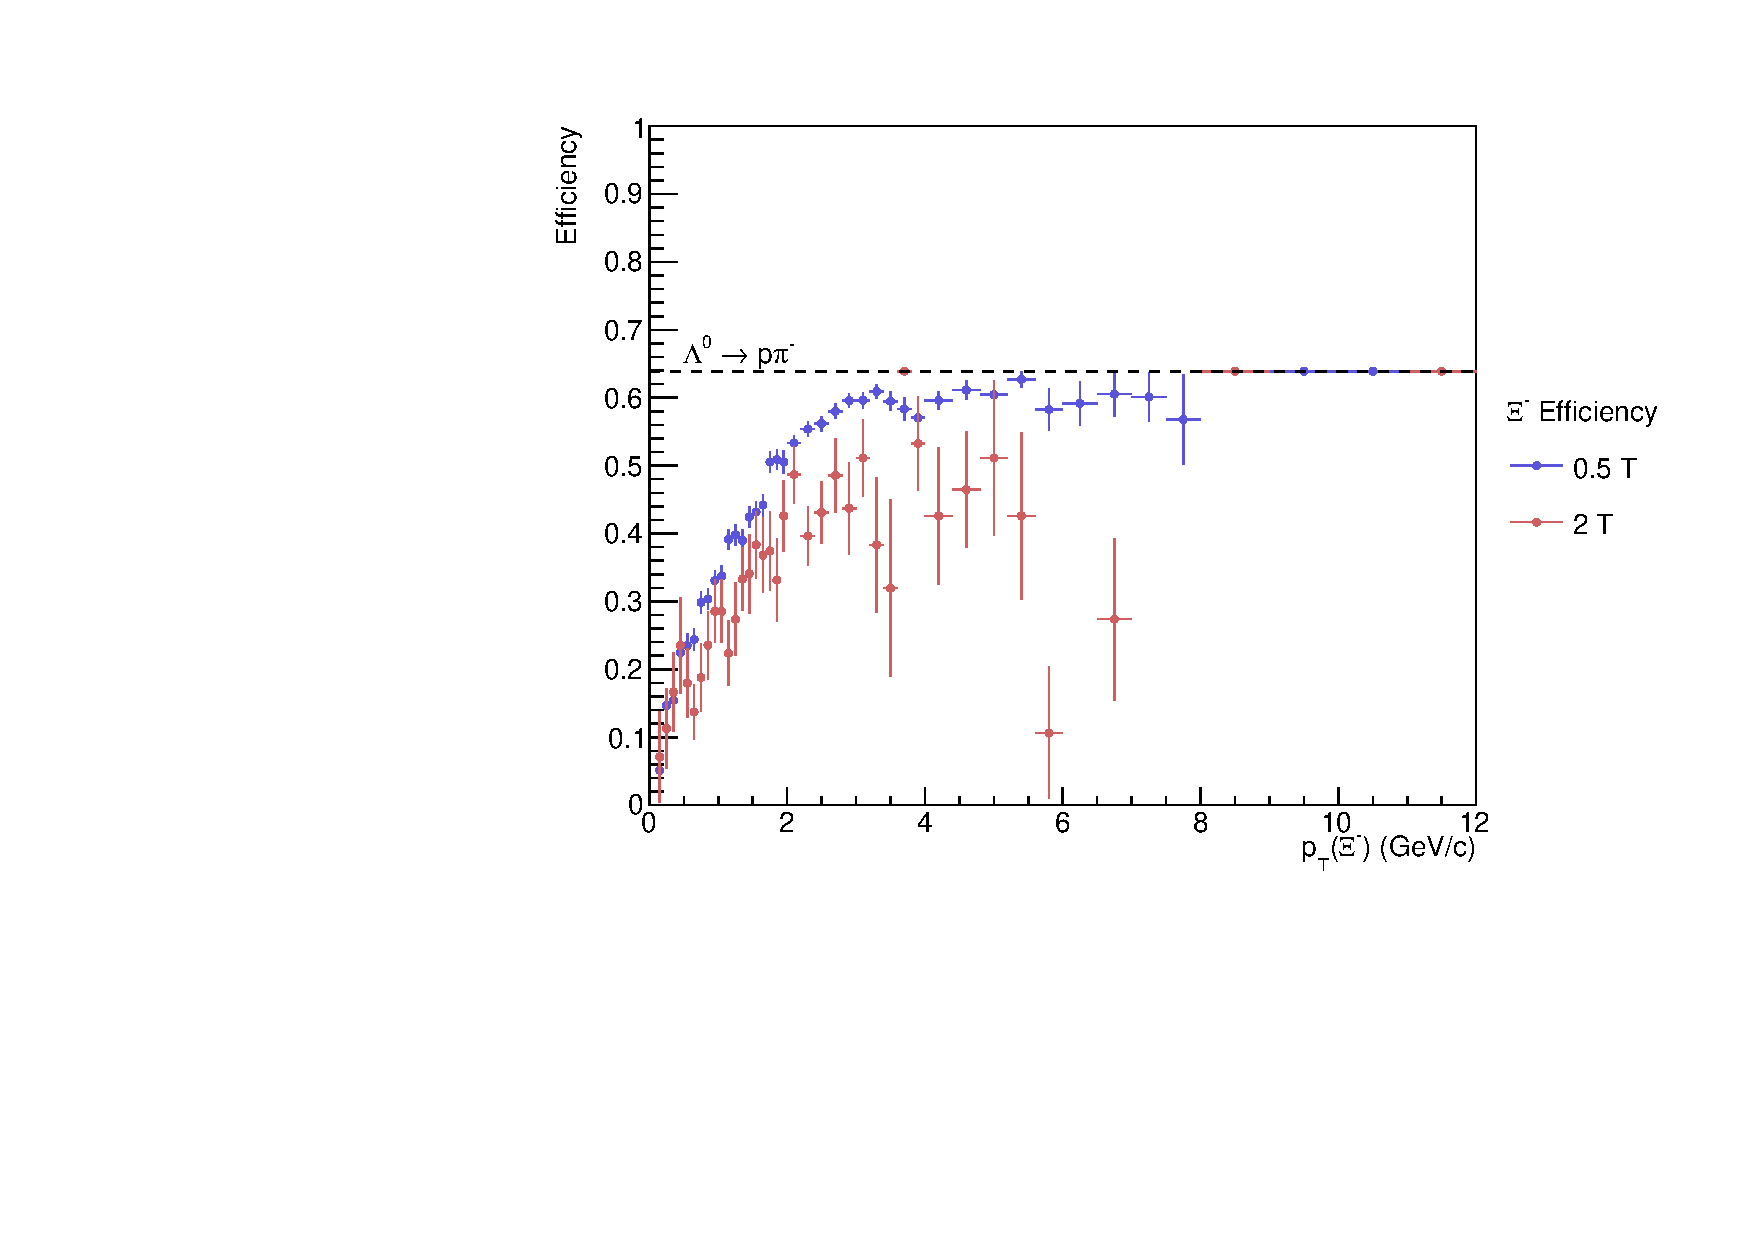
\includegraphics[width=1\linewidth]{smi-template/XiEffVsPt.pdf}
            \caption{My figure text}
            \label{fig:enter-label}
        \end{figure}
    \end{minipage}
\end{frame}
\end{document}
